\documentclass[11pt,a4paper,oneside]{article}

\usepackage[T1]{fontenc}
\usepackage[utf8]{inputenc}
\usepackage{lmodern}
\usepackage{microtype}
\usepackage[a4paper,margin=26mm,headheight=15pt]{geometry}
\usepackage{amsmath,amssymb,mathtools}
\usepackage{graphicx}
\usepackage{booktabs}
\usepackage{tabularx}
\usepackage{longtable}
\usepackage{array}
\usepackage{ragged2e}
\usepackage{enumitem}
\usepackage{xcolor}
\usepackage{caption}
\usepackage{float}
\usepackage{placeins}
\usepackage{pdflscape}
\usepackage{fancyhdr}
\usepackage{tcolorbox}
\usepackage{listings}
\usepackage{csquotes}
\usepackage[backend=bibtex,style=numeric,sorting=none,maxbibnames=20]{biblatex}
\usepackage[colorlinks=true,linkcolor=AEGBlue,citecolor=AEGBlue,urlcolor=AEGBlue]{hyperref}
\usepackage[capitalise,noabbrev]{cleveref}

\definecolor{AEGInk}{HTML}{0E223D}
\definecolor{AEGOrange}{HTML}{B74318}
\definecolor{AEGBlue}{HTML}{236BAA}
\definecolor{AEGGreen}{HTML}{28735C}
\definecolor{AEGAmber}{HTML}{8B6508}
\definecolor{EvidenceGray}{HTML}{666666}
\definecolor{CalloutFill}{HTML}{FFF4EE}
\definecolor{BoundaryFill}{HTML}{FFF8E8}

\addbibresource{references.bib}
\graphicspath{{figures/}}

\setlength{\parindent}{0pt}
\setlength{\parskip}{0.58em}
\setlength{\emergencystretch}{1.5em}
\setcounter{secnumdepth}{3}
\setcounter{tocdepth}{2}
\setlist[itemize]{leftmargin=1.5em,itemsep=0.25em,topsep=0.25em}
\setlist[enumerate]{leftmargin=1.7em,itemsep=0.25em,topsep=0.25em}
\captionsetup{font=small,labelfont=bf,justification=justified,singlelinecheck=false}

\newcommand{\evidence}[1]{\textsuperscript{\textcolor{EvidenceGray}{[#1]}}}
\newcommand{\competition}{\textsuperscript{\textcolor{EvidenceGray}{[C1]}}}
\newcommand{\fixedtablecaption}[3]{%
  \par\smallskip\phantomsection\hypertarget{#1}{}\label{#1}\begin{minipage}{\linewidth}\small\textbf{Table #2.} #3\end{minipage}\par\smallskip}
\newcommand{\tableref}[2]{\hyperlink{#1}{Table #2}}
\newcommand{\sectionlead}[1]{\begin{quote}\itshape #1\end{quote}}
\newcommand{\R}{\mathbb{R}}

\newcolumntype{Y}{>{\RaggedRight\arraybackslash}X}
\newcolumntype{L}[1]{>{\RaggedRight\arraybackslash}p{#1}}
\newcolumntype{C}[1]{>{\Centering\arraybackslash}p{#1}}

\tcbset{
  boxrule=0.7pt,
  arc=1.2mm,
  left=3mm,right=3mm,top=2.5mm,bottom=2.5mm,
  before skip=0.7em,after skip=0.7em
}
\newtcolorbox{evidencebox}{colback=CalloutFill,colframe=AEGOrange}
\newtcolorbox{boundarybox}{colback=BoundaryFill,colframe=AEGAmber}

\pagestyle{fancy}
\fancyhf{}
\fancyhead[L]{\small\textsc{AegisLoop}}
\fancyhead[R]{\small Mastercard Innovation Challenge 2026}
\fancyfoot[C]{\thepage}
\renewcommand{\headrulewidth}{0.4pt}
\renewcommand{\footrulewidth}{0pt}
\fancypagestyle{plain}{\fancyhf{}\fancyfoot[C]{\thepage}\renewcommand{\headrulewidth}{0pt}}

\lstdefinestyle{aegiscode}{
  basicstyle=\ttfamily\footnotesize,
  frame=single,
  rulecolor=\color{black!25},
  backgroundcolor=\color{black!2},
  breaklines=true,
  columns=fullflexible,
  showstringspaces=false
}

\begin{document}

\begin{titlepage}
  \thispagestyle{empty}
  \centering
  \vspace*{13mm}
  {\small\bfseries\color{AEGOrange} MASTERCARD INNOVATION CHALLENGE 2026\par}
  \vspace{17mm}
  {\fontsize{36}{40}\selectfont\bfseries\color{AEGInk} AegisLoop\par}
  \vspace{4mm}
  {\Large Closing the loop between emerging payment-fraud campaigns and adaptive defense\par}
  \vspace{10mm}
  {\color{AEGOrange}\rule{0.72\textwidth}{1.2pt}\par}
  \vspace{14mm}
  {\large\bfseries An evidence-locked solution walkthrough and technical research paper\par}
  \vfill
  \begin{tabular}{rl}
    \textbf{Author:} & Abhishek Das \\
    \textbf{Programme:} & Fourth-year undergraduate, Department of Chemical Engineering \\
    \textbf{Institution:} & Indian Institute of Technology Guwahati \\
    \textbf{Competition:} & Mastercard Innovation Challenge 2026 \\
    \textbf{Track:} & AI Defense Lab for Payment Security \\
    \textbf{Date:} & August 2026
  \end{tabular}
  \vfill
  \begin{minipage}{0.82\textwidth}
    \centering\small
    \textbf{Working prototype:} \url{https://aegisloop-mcic-2026.vercel.app}\\[2mm]
    \textbf{Repository:} \url{https://github.com/Hermes-25/AegisLoop}
  \end{minipage}
  \par
  \vspace{9mm}
  {\footnotesize The full technical paper is the primary evidence document for the submission. All quantitative claims trace to the approved versioned artifacts listed in Appendix B.\par}
\end{titlepage}

\pagenumbering{roman}
\begin{abstract}
Payment-fraud defenses are usually evaluated against a fixed attack set, while adversaries adapt after each control change. AegisLoop turns that asymmetry into a controlled learning loop: it identifies eight equal-priority GenAI-enabled fraud archetypes and 32 variants; generates stateful, entity-linked synthetic campaigns behind a fidelity firewall; uses a LinUCB contextual bandit to select complete campaign parameters; and hardens a supervised, unsupervised and relational-risk defender on valid evasions. In the fixed five-seed full protocol, the bandit achieved mean reward 0.807 (95\% CI 0.519--1.212), exceeding random search on every paired seed (mean difference 0.681; one-sided paired Wilcoxon $p=0.03125$). Held-out-family ROC-AUC rose from 0.9806 at V0 to 0.99993 at V2, while recall rose from 86.59\% to 99.90\%. Against a matched, fixed action pool held constant across generations, the hardened defender (V2) detected every campaign across five seeds. The central caveat is operationally important: V2 precision falls from 90.17\% at 9.39\% laboratory prevalence to 1.31\% when the same scores are reweighted to 0.015\% prevalence (seed 20260812; full range in Appendix Table A3). The contribution is therefore not a production detector claim; it is a reproducible campaign-level extension of single-transaction RL evasion that closes the loop into adversarial defender hardening.\evidence{E1--E6}
\end{abstract}

\noindent\textbf{Index Terms:} payment fraud, adversarial machine learning, contextual bandits, synthetic data, model risk management.

\begin{evidencebox}
\textbf{Decision in one sentence.} Use AegisLoop as an offline, governed threat laboratory that finds campaign-level blind spots before they become production losses - with evidence boundaries made explicit.
\end{evidencebox}

\tableofcontents
\listoffigures
\section*{List of Tables}
\addcontentsline{toc}{section}{List of Tables}
\noindent\tableref{tab:headline}{1}. Headline results \dotfill \pageref{tab:headline}\\
\tableref{tab:ablation}{2}. Reward ablation \dotfill \pageref{tab:ablation}\\
\tableref{tab:split}{3}. Temporal split and calibration contract \dotfill \pageref{tab:split}\\
\tableref{tab:roles}{4}. Attack-family roles \dotfill \pageref{tab:roles}\\
\tableref{tab:fidelity}{5}. Campaign-diagnostic summary \dotfill \pageref{tab:fidelity}\\
\tableref{tab:defender}{6}. Defender ensemble design \dotfill \pageref{tab:defender}\\
\tableref{tab:efficacy}{7}. Held-out-family results \dotfill \pageref{tab:efficacy}\\
\tableref{tab:deployment}{8}. Directional deployment path \dotfill \pageref{tab:deployment}
\clearpage

\pagenumbering{arabic}

\section{Introduction}
\sectionlead{The material problem is not detecting yesterday's fraud; it is creating a safe, measurable loop in which new attack hypotheses expose gaps and those gaps improve the next defender.}

The challenge asks teams to identify novel fraud attacks, generate high-fidelity simulations, build effective mitigations and demonstrate real-world feasibility. It also states that defense gaps should feed new attack ideas. AegisLoop treats those requirements as one system rather than four disconnected artifacts.\competition

\subsection{The three-pillar problem}
\begin{itemize}
  \item \textbf{Identify:} maintain a structured attack atlas that spans authorization, account-to-account, identity, merchant and post-transaction abuse.
  \item \textbf{Generate:} compile each hypothesis into an ordered, entity-linked synthetic campaign whose validity can be checked before it receives reward.
  \item \textbf{Defend:} let an adaptive policy probe a frozen detector, then retrain and recalibrate only at an explicit governance boundary.
\end{itemize}

\subsection{Falsifiable hypotheses}
The evaluation tests four explicit hypotheses under the fixed protocol; they are not claims inferred after looking at a single favorable seed.\evidence{E1,E2,E8}
\begin{itemize}
  \item \textbf{H1 - Adaptive search:} with the defender, action pool and campaign budget held fixed, LinUCB produces higher mean campaign reward than random search and rule mutation.
  \item \textbf{H2 - Adversarial hardening:} training on fidelity-valid evasions improves held-out-family ranking and recall from V0 through the hardened generations without using the test split for threshold selection.
  \item \textbf{H3 - Later-generation stability:} a second hardening transition does not increase matched-pool fresh-attacker reward relative to V1; with five seeds, this test is directional and low-powered.
  \item \textbf{H4 - Novelty contribution:} zeroing the novelty bonus changes attacker reward; the two-sided test permits a positive, negative or null answer.
\end{itemize}

\subsection{Contributions}
\begin{enumerate}
  \item A campaign-level attack representation: actions select a family plus intensity, timing, reuse and evasion parameters, rather than perturbing one transaction feature at a time.\evidence{E7}
  \item A hand-coded, stateful payment digital twin that preserves chronology and entity reuse by construction, avoiding the structural limitations of row-independent generators without claiming real-data fidelity.\evidence{E7}\cite{sajja2026synthetic}
  \item A tractable contextual-bandit formulation with immediate campaign reward, equal-budget baselines and per-term reward logging.\evidence{E1,E2,E7,E8}
  \item A leakage-controlled V0--V1--V2 hardening protocol with final held-out families, validation-only threshold calibration and raw campaign diagnostics.\evidence{E1--E5,E8}
  \item A negative-result discipline: the novelty reward term is inert, the V1--V2 stability result is directional rather than conclusive, and deployment-prevalence precision collapses.\evidence{E1,E4}
\end{enumerate}

\section{Related Work and Precise Positioning}
\sectionlead{AegisLoop does not claim to invent RL evasion, contextual bandits or relational fraud scoring; its defensible novelty is connecting those ideas at the campaign and defender-generation levels.}

\subsection{FRAUD-RLA: adversarial-RL precedent}
Lunghi et al. formulate reinforcement-learning attacks that bypass credit-card fraud classifiers under constrained attacker knowledge. AegisLoop adopts the adversarial learning premise but changes the unit of action: the policy selects a complete, linked campaign rather than only feature-level evasion for a transaction. It then carries successful, fidelity-valid evasions across a governed boundary into defender hardening.\evidence{E7}\cite{lunghi2025fraudrla}

\subsection{Adyen: bandit precedent and instability warning}
Vangara and Egg analyze contextual bandits in payment processing, including non-uniform exploration, delayed feedback and later-generation instability. Their application optimizes payment decisions; AegisLoop uses LinUCB adversarially to choose attack campaigns. The study's warning about reward-distribution shift is why AegisLoop tests a second hardening transition instead of stopping at V1.\evidence{E1,E8}\cite{vangara2024contextual}

\subsection{Sajja: structural limits of row-independent synthesis}
Sajja shows that row-independent tabular generators are structurally unable to preserve multi-account graph motifs and positive within-entity inter-event-time autocorrelation. AegisLoop therefore uses a PaySim-style agent simulation that binds entities once and evolves sequences. This is a design justification, not evidence that the synthetic campaigns match real fraud; no real reference corpus is used.\evidence{E7}\cite{sajja2026synthetic}

\subsection{Mastercard Decision Intelligence Pro: deployment direction}
Mastercard describes Decision Intelligence Pro as real-time decisioning that connects account, purchase, merchant and device relationships. AegisLoop does not claim equivalence to DI Pro and uses no published Mastercard performance number as a benchmark. The alignment is architectural: entity relationships and transaction context should enrich an issuer or network score, while AegisLoop remains an offline pre-production red-team laboratory.\evidence{E7}\cite{mastercard2024dipro}

\begin{table}[H]
\centering\small
\begin{tabularx}{\linewidth}{L{31mm}YY}
\toprule
\textbf{Reference} & \textbf{What it establishes} & \textbf{AegisLoop's distinct scope} \\
\midrule
FRAUD-RLA & RL can evade fraud classifiers & Campaign-level, entity-linked actions plus hardening \\
Adyen bandits & Industrial bandit trade-offs and instability & Adversarial search; explicit V1--V2 check \\
Sajja & Limits of row-independent synthesis & Stateful hand-coded simulation; no fidelity proof \\
Mastercard DI Pro & Relational, contextual risk direction & Offline discovery feeds governed score enhancement \\
\bottomrule
\end{tabularx}
\caption*{Positioning against the five-reference public evidence base.}
\end{table}

\begin{landscape}
\begin{figure}[p]
  \centering
  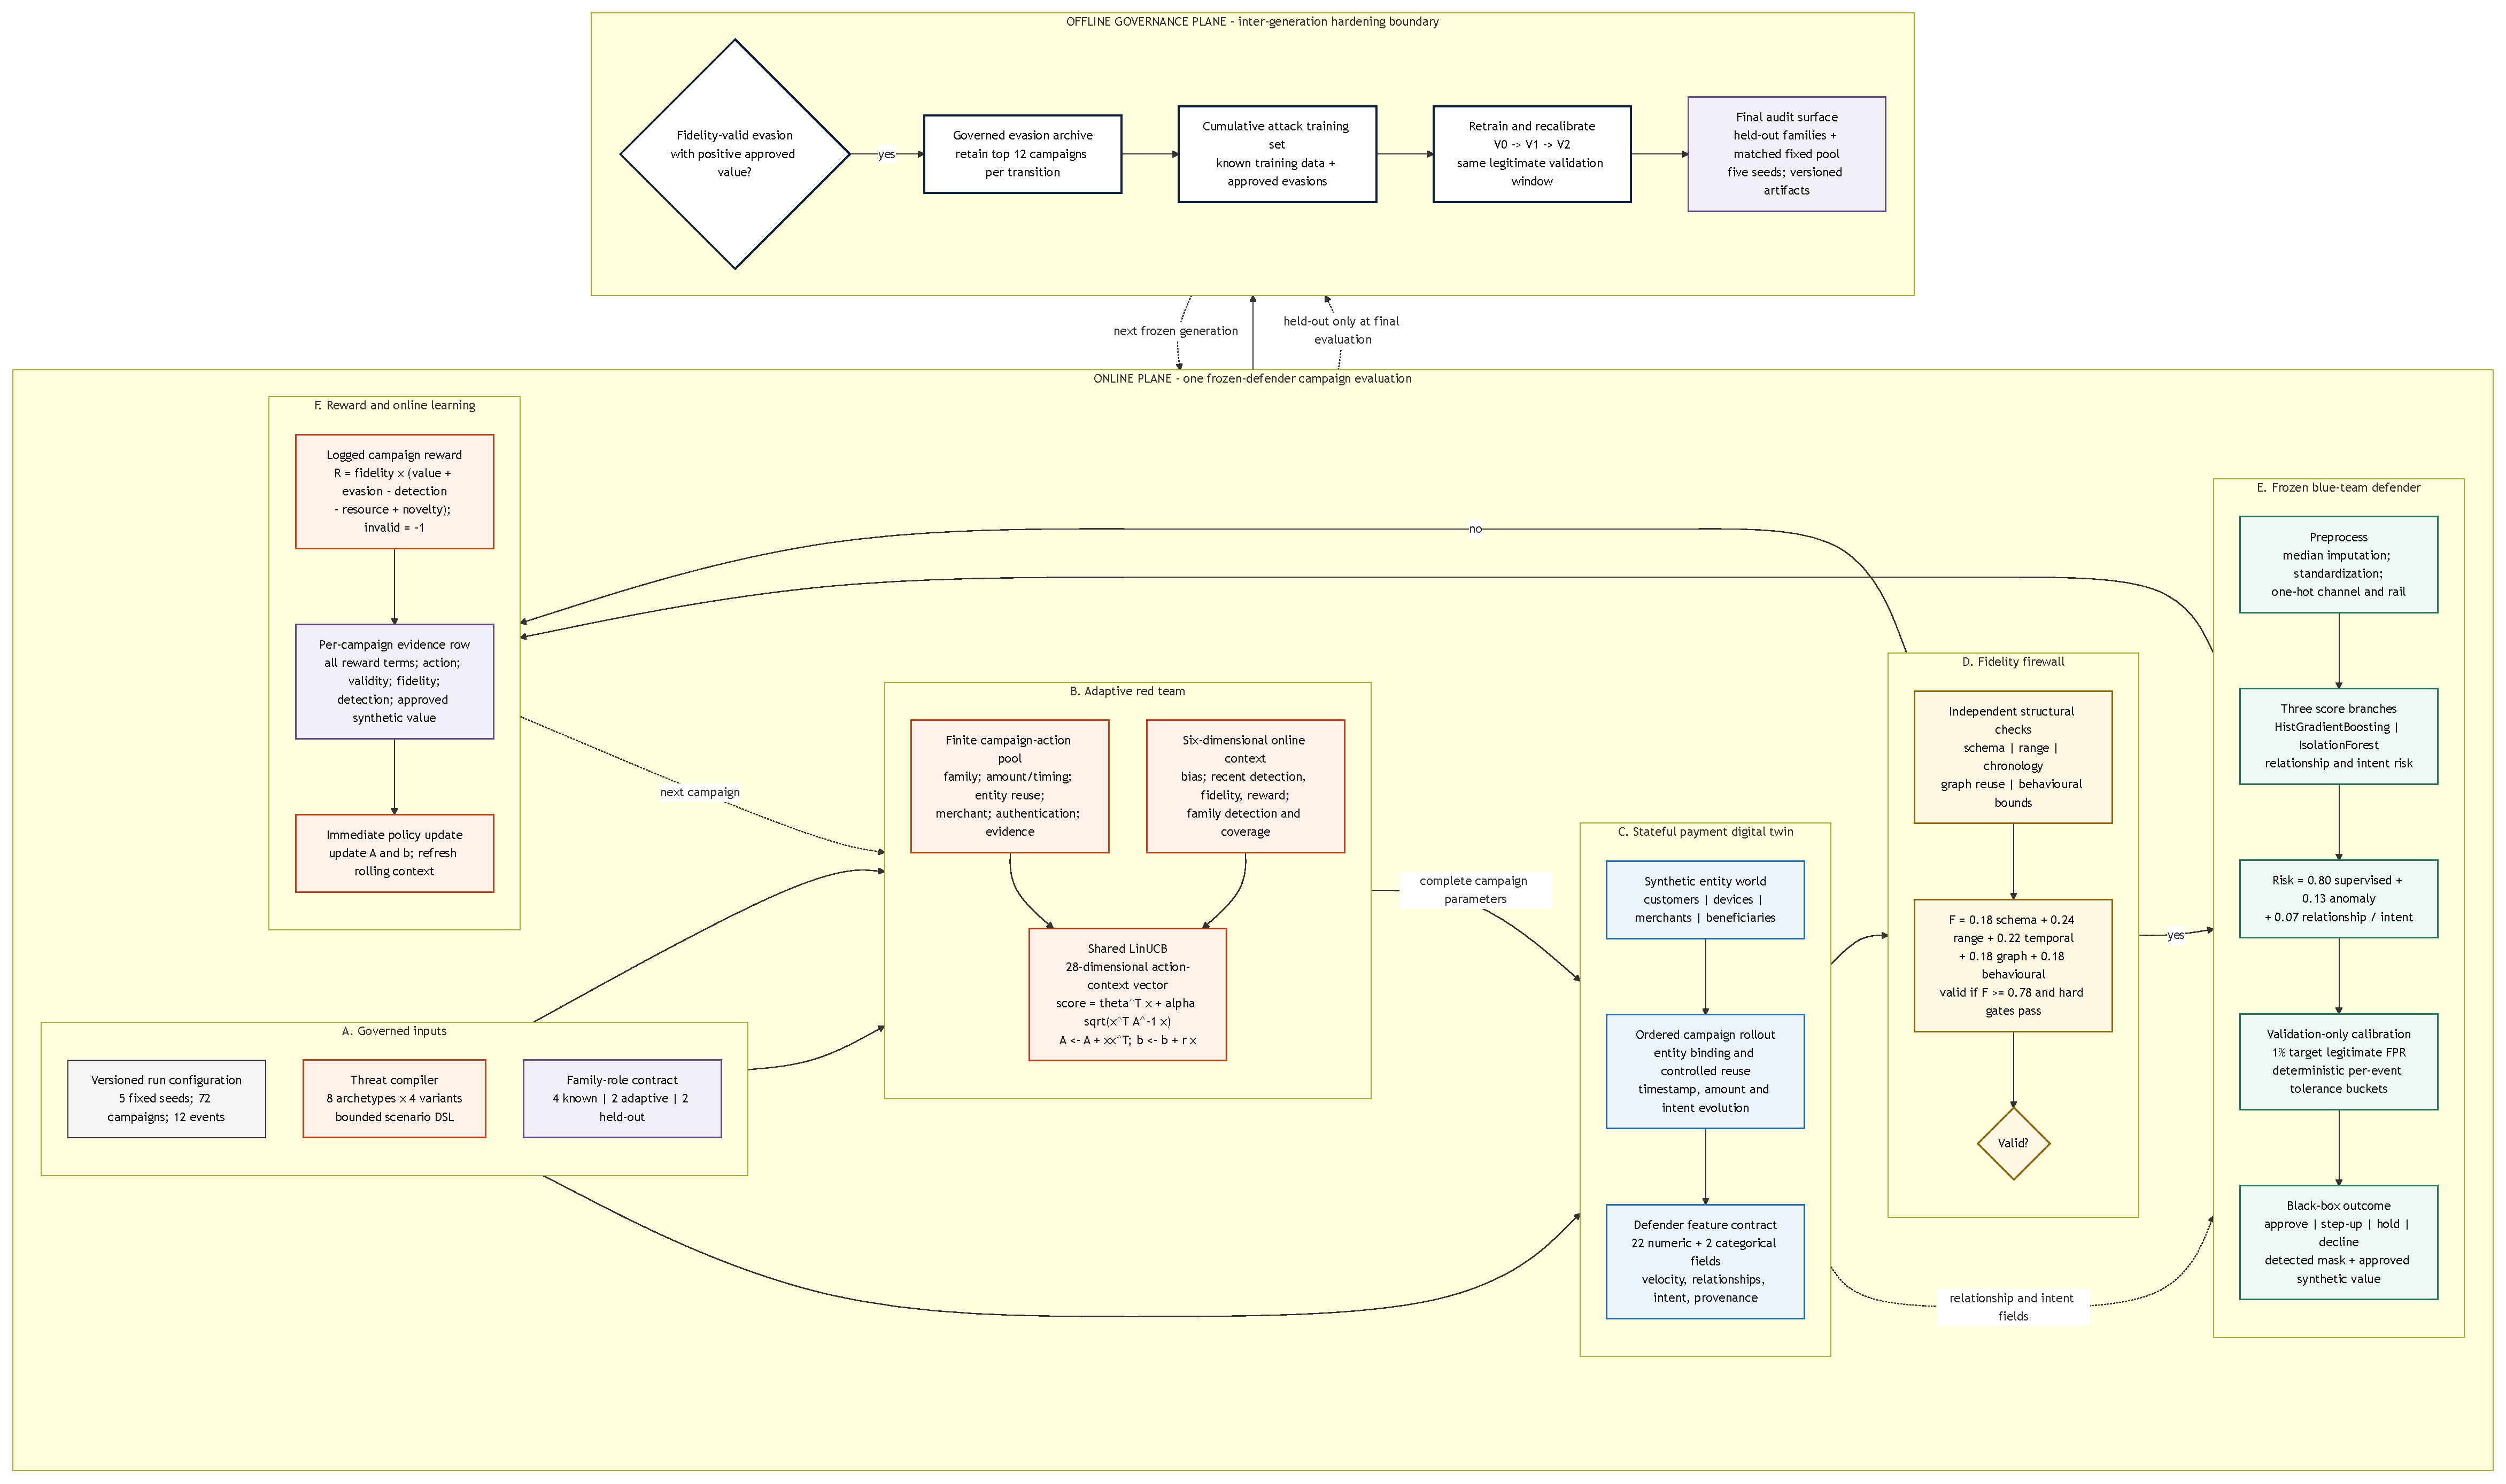
\includegraphics[width=0.98\linewidth,height=0.82\textheight,keepaspectratio]{fig01_technical_architecture.pdf}
  \caption[Detailed technical architecture]{Detailed AegisLoop technical architecture. The online plane evaluates one complete campaign against a frozen defender and returns an immediate scalar reward to LinUCB. The offline governance plane admits only fidelity-valid, positive-value evasions, then retrains and recalibrates the next defender generation. The diagram is generated locally from Mermaid source and grounded in the implementation and benchmark contracts.\evidence{E7,E8}}
  \label{fig:architecture}
\end{figure}
\end{landscape}

\section{Identify: Threat Landscape}
\sectionlead{The atlas is deliberately broad and symmetric: all eight archetypes are first-class hypotheses, while three case studies simply make the mechanics concrete.}

\begin{figure}[H]
  \centering
  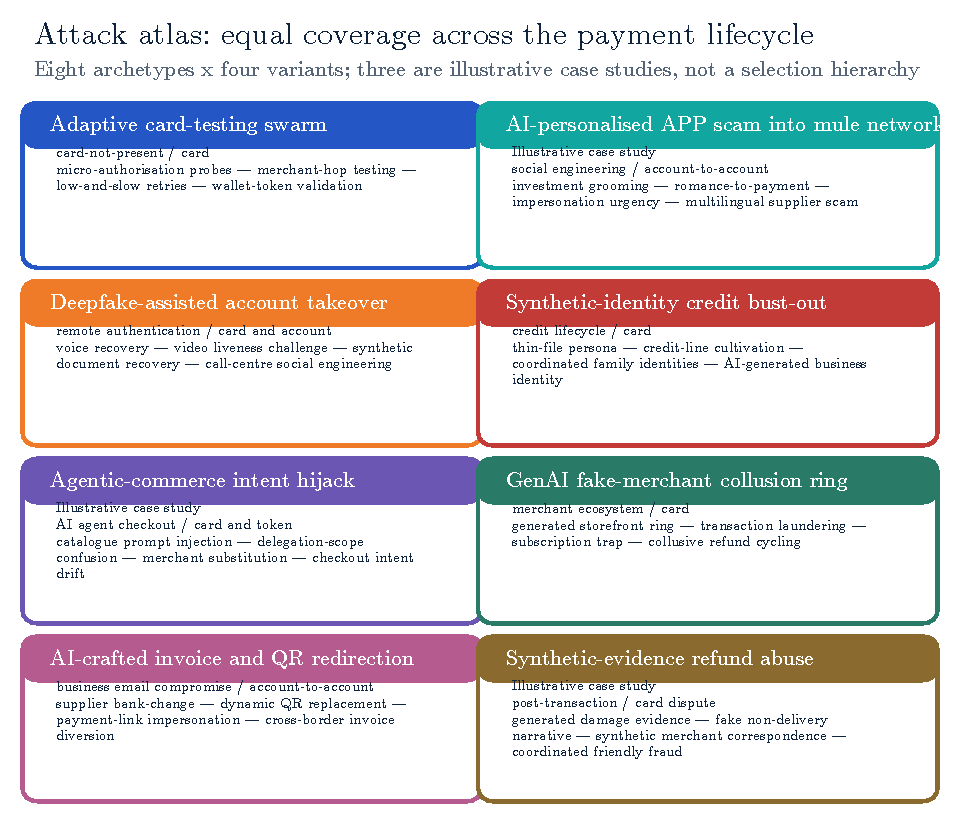
\includegraphics[width=\linewidth]{fig02_attack_atlas.pdf}
  \caption[Attack atlas and taxonomy]{Attack atlas and taxonomy. All labels and variants are generated from \texttt{attack\_atlas.json}; all eight archetypes have equal status.\evidence{E6}}
  \label{fig:atlas}
\end{figure}

\subsection{How to read the atlas}
\Cref{fig:atlas} separates the attack objective from the channel and payment rail through which it unfolds. Each archetype owns four bounded variants and an ordered event-sequence template. The atlas therefore defines a reproducible hypothesis space rather than a free-form prompt catalogue. Equal visual weighting prevents the three illustrative cases below from being misread as the only important threats.

\subsection{Three illustrative case studies}
\textbf{Agentic-commerce intent hijack.} A delegated shopping agent begins with legitimate user intent, encounters poisoned catalogue or merchant context, drifts outside its scope and completes checkout. The defense implication is verifiable intent and action traceability, not only transaction anomaly scoring. Its four approved variants are hidden instruction drift, poisoned product metadata, scope escalation checkout and delegated-agent credential misuse.\evidence{E6}

\textbf{AI-personalised APP scam into a mule network.} An LLM-assisted pretext sustains trust, introduces a new payee, tests a small transfer and escalates value. The event sequence lets the simulator expose beneficiary reuse and behavioral step-up signals across account-to-account payments.\evidence{E6}

\textbf{Synthetic-evidence refund abuse.} A legitimate purchase and fulfilment are followed by forged damage or non-delivery evidence and a refund claim. The control surface shifts to evidence provenance, claim history and merchant fulfilment signals after authorization.\evidence{E6}

\begin{boundarybox}
\textbf{Safety boundary.} These are synthetic research patterns. The system contains no cardholder data, credentials or live-payment connector; the attack atlas is compiled into bounded simulation parameters rather than exposed as a free-form attack service.\competition\evidence{E7}
\end{boundarybox}

\begin{table}[H]
\centering\small
\begin{tabularx}{\linewidth}{L{28mm}C{14mm}YY}
\toprule
\textbf{Family role} & \textbf{Count} & \textbf{Permitted use} & \textbf{Leakage control} \\
\midrule
Known & 4 & Supervised train, validation and test campaigns & Campaign-disjoint partitions \\
Adaptive search & 2 & Bandit search and hardening & Absent from initial supervised data \\
Final held-out & 2 & V0, V1 and V2 generalization evaluation & Never enters search, training or calibration \\
\bottomrule
\end{tabularx}
\fixedtablecaption{tab:roles}{4}{Attack-family roles.\evidence{E7,E8}}
\end{table}

\section{System Architecture}
\sectionlead{AegisLoop is an offline closed loop with separable responsibilities for governed inputs, safe campaign generation, adaptive search, frozen scoring, immediate reward and inter-generation hardening.}

\Cref{fig:architecture} is the implementation architecture, not a conceptual loop. It makes two boundaries explicit. The \emph{online plane} evaluates one campaign while the defender remains frozen. The \emph{offline governance plane} changes the defender only after eligible evasions are archived. That separation prevents the attacker from silently changing the object being evaluated.

\subsection{Governed inputs and role isolation}
A versioned configuration fixes five seeds, a 72-campaign budget and 12 events per evaluation. The threat compiler transforms eight archetypes and four variants per archetype into a finite scenario DSL. Family roles are resolved before training: four known families may enter supervised data, two adaptive families drive red-team search, and two final-held-out families are excluded from search, fitting and calibration.\evidence{E6--E8}

\subsection{Campaign policy and feature construction}
At campaign $t$, LinUCB receives a six-dimensional context
\[
  c_t = [1,\ \bar d_t,\ \bar f_t,\ \bar r_t/5000,\ \bar d_{t,k},\ q_{t,k}]^\top,
\]
where $\bar d_t$, $\bar f_t$ and $\bar r_t$ summarize recent detection, fidelity and reward, while $\bar d_{t,k}$ and $q_{t,k}$ summarize detection and coverage for family $k$. Each candidate action adds an eight-family one-hot representation, seven bounded continuous parameters and seven context-action interactions, producing a 28-dimensional vector $x_{t,a}\in\R^{28}$. The shared linear upper-confidence policy selects
\begin{align}
  \hat\theta_t &= A_t^{-1}b_t, \\
  a_t &= \arg\max_a \left(x_{t,a}^\top\hat\theta_t + \alpha\sqrt{x_{t,a}^\top A_t^{-1}x_{t,a}}\right), \qquad \alpha=1.15, \\
  A_{t+1} &= A_t + x_{t,a_t}x_{t,a_t}^\top, \qquad b_{t+1}=b_t+r_tx_{t,a_t}.
\end{align}
This is lightweight RL: the action is a complete campaign configuration and the feedback is immediate, so a long-horizon value function is neither assumed nor required.\evidence{E7,E8}

\subsection{Stateful digital twin and event contract}
The selected action binds customers, devices, merchants and beneficiaries into one ordered campaign. Entity reuse is controlled by the action but resolved by the simulator, so velocity, graph degree, relationship reuse, intent and provenance evolve from preceding events. The emitted defender contract contains 22 numeric and two categorical fields, including channel and rail. This preserves chronology and shared-entity motifs by construction rather than sampling rows independently.\evidence{E7}

\subsection{Fidelity firewall}
The firewall evaluates schema, range, temporal, graph and behavioral checks independently. Its composite score is
\[
  F = 0.18F_{schema}+0.24F_{range}+0.22F_{temporal}+0.18F_{graph}+0.18F_{behavioral}.
\]
A campaign is valid only when $F\geq0.78$ and the schema, range and temporal hard gates pass. Invalid campaigns receive reward $-1$ with zeroed reward components. The firewall cannot read detector probabilities or thresholds; it prevents malformed synthetic traffic from earning reward but does not prove real-data equivalence.\evidence{E5,E7}

\subsection{Frozen defender ensemble}
The preprocessor median-imputes and standardizes numeric features and one-hot encodes channel and rail. The score combines a supervised \texttt{HistGradientBoostingClassifier}, an \texttt{IsolationForest} fitted only on legitimate training events, and a relationship/intent branch:
\[
  s(x)=0.80s_{sup}(x)+0.13s_{anom}(x)+0.07s_{rel}(x).
\]
Each generation calibrates its decision threshold only on the legitimate validation window at a 1\% target false-positive rate. Deterministic per-event tolerance buckets map the score to approve, step-up, hold or decline outcomes; the attacker observes only the resulting detected mask and approved synthetic value.\evidence{E3,E7}

\subsection{Reward trace and hardening boundary}
Every campaign writes the chosen action, validity, fidelity, each reward component, detection rate and approved synthetic value. Only fidelity-valid evasions with positive approved value may enter the top-12 governed archive for a generation transition. The next training set is cumulative, but legitimate validation data is unchanged and the held-out test remains untouched. This yields two actual hardening transitions, V0--V1 and V1--V2.\evidence{E3,E5,E7,E8}

\section{Generate: Stateful Simulation and Fidelity}
\sectionlead{AegisLoop chooses controllable structural fidelity over untestable realism: campaigns are stateful and entity-linked by construction, while no claim is made that they reproduce a real portfolio distribution.}

\subsection{Simulator design}
The hand-coded agent simulation creates 2,400 customers, 620 merchants, 2,900 devices and 1,300 beneficiaries, then emits 28,000 legitimate events before campaign generation. It binds entities to a scenario and rolls out ordered events with campaign lengths bounded from five to twenty; the full evaluation uses twelve events. Timestamps, amount trajectories, velocity aggregates, reuse counts and relationship features evolve with the campaign. It is not CTGAN, TVAE, GaussianCopula, TabularARGN or another learned row-independent generator.\evidence{E7,E8}

\subsection{Representative campaign mechanics}
The versioned representative agentic-checkout rollout contains nine chronologically ordered events and an entity footprint of eight devices, five merchants and seven beneficiaries. Those counts are not arbitrary summary labels: the selected action sets device reuse to 0.3493 and beneficiary reuse to 0.3060, and the simulator applies those probabilities at each later event. Repeated entities create shared graph motifs, while new entities model controlled churn. Per-event velocity measures count recent actions in the preceding window; graph degree counts entity connections; relationship reuse indicates whether a device, merchant or beneficiary has appeared earlier in the same linked history.\evidence{E7}

\subsection{V2 fidelity diagnostic}
The post-approval diagnostic rules out the trivial explanation that V2 received zero approved value because its campaigns failed validation. Every V2 campaign is valid; the table reports fidelity and action diversity directly from the 360-row artifact.\evidence{E5}

\begin{table}[H]
\centering\small
\begin{tabular}{ccccc}
\toprule
\textbf{Seed} & \textbf{Valid} & \textbf{Mean fidelity} & \textbf{Minimum fidelity} & \textbf{Unique actions} \\
\midrule
20260812 & 72/72 & 0.927 & 0.837 & 33 \\
20260813 & 72/72 & 0.918 & 0.838 & 32 \\
20260814 & 72/72 & 0.919 & 0.824 & 37 \\
20260815 & 72/72 & 0.927 & 0.837 & 31 \\
20260816 & 72/72 & 0.924 & 0.831 & 37 \\
\bottomrule
\end{tabular}
\fixedtablecaption{tab:fidelity}{5}{Campaign-diagnostic summary. Each seed contains 72 campaigns and 864 events.\evidence{E5}}
\end{table}

The score means that a campaign passed the implemented schema, range, chronology, behavioral and entity-reuse checks. It does not mean the campaign matches an issuer's marginal distribution, temporal signature or fraud-loss rate; those claims require authorized reference data and external validation.\evidence{E7}\cite{sajja2026synthetic}

\section{Adapt: Contextual-Bandit Red Team}
\sectionlead{The attacker is genuine lightweight RL: a contextual bandit learns which complete campaign configuration to try next from immediate black-box defender feedback.}

\subsection{Why a contextual bandit, not a full MDP}
Each decision chooses one complete 12-event campaign from a finite action pool and receives an immediate scalar reward after the frozen defender scores it. There is no need to estimate delayed long-horizon value; LinUCB supplies transparent exploration and exploitation with a small data budget. The state summarizes recent detector outcomes; the action encodes attack family and bounded intensity, timing, reuse and evasion parameters.\evidence{E7,E8}

\subsection{Reward specification}
For a valid campaign, the logged reward is
\begin{equation}
R = F\left(\frac{V}{500}+2.5(1-D)-0.16D-2.5\frac{N}{1000}+0.20I_{novel}\right),
\label{eq:reward}
\end{equation}
where $F\in[0,1]$ is fidelity, $V$ is approved synthetic value, $D$ is event detection rate, $N$ is campaign event count and $I_{novel}$ marks the first successful discretized pattern. Invalid campaigns receive $-1$ and zero component terms. The coefficients are fixed engineering design priors, not weights fitted to the five reported seeds: $V/500$ puts hundreds of approved-value units on the evasion scale; $2.5$ makes full evasion the dominant objective; $-0.16D$ penalizes detection; $-2.5N/1000$ charges 0.0025 per event to discourage gratuitous length; and the 0.20 novelty bonus is deliberately subordinate to evasion. Every term, pre-fidelity reward and final reward is logged per campaign.\evidence{E7--E9}

\subsection{Novelty ablation}
\begin{table}[H]
\centering\small
\begin{tabular}{lccc}
\toprule
\textbf{Full five-seed ablation} & \textbf{Mean reward} & \textbf{SD} & \textbf{Bootstrap 95\% CI} \\
\midrule
Novelty on & 0.807 & 0.457 & [0.519, 1.212] \\
Novelty zeroed & 0.824 & 0.349 & [0.574, 1.105] \\
Paired on minus off & -0.017 & 0.159 & [-0.137, 0.121] \\
\bottomrule
\end{tabular}
\fixedtablecaption{tab:ablation}{2}{Reward ablation. Two-sided paired Wilcoxon $p=0.625$; novelty is not a performance driver.\evidence{E1,E2}}
\end{table}

The novelty component is instrumented, not credited with performance. Its null result is reported with the same prominence as the positive attacker result because it narrows the defensible explanation: approved value, evasion and controlled exploration drive the result; the 0.20 novelty bonus does not.\evidence{E1,E2}

\section{Defend: Ensemble and Hardening}
\sectionlead{The blue team combines complementary signals, then recalibrates each hardened generation on the same disjoint validation window before any test metric is computed.}

\begin{table}[H]
\centering\small
\begin{tabularx}{\linewidth}{L{38mm}L{48mm}Y}
\toprule
\textbf{Layer} & \textbf{Role} & \textbf{Why it matters} \\
\midrule
Supervised gradient boosting & Learn labeled tabular interactions & Strong known-pattern baseline and ranking \\
Isolation scoring & Surface distributional outliers & Covers unusual behavior without an attack label \\
Relationship and intent risk & Encode entity reuse and delegated-intent inconsistency & Captures campaign structure beyond one row \\
Policy action & Approve, step-up, hold or decline & Maps score to an operational response vocabulary \\
\bottomrule
\end{tabularx}
\fixedtablecaption{tab:defender}{6}{Defender ensemble design.\evidence{E7}}
\end{table}

\subsection{Governed hardening}
A successful red-team campaign must be fidelity-valid, produce positive approved synthetic value and evade at least part of the frozen defender. Only then can it enter the next defender's training data. Validation legitimate traffic remains unchanged, each generation computes its own threshold and test traffic remains untouched. This creates two real transitions, V0--V1 and V1--V2, without test-set feedback.\evidence{E3,E7,E8}

\subsection{Operational separation}
In a production architecture, AegisLoop outputs scenario definitions, validated synthetic campaigns, feature-gap findings and candidate challenger data. A network or issuer decision engine remains the system of record. AegisLoop does not sit in the authorization path and makes no live approve-or-decline decision.\evidence{E7}

\section{Experimental Methodology}
\sectionlead{The evidence protocol is paired, seed-robust and leakage-controlled; its remaining weakness is statistical scale, not hidden test reuse.}

\subsection{Temporal split and calibration contract}
\begin{table}[H]
\centering\small
\begin{tabularx}{\linewidth}{L{24mm}C{24mm}C{25mm}Y}
\toprule
\textbf{Split} & \textbf{Legitimate rows} & \textbf{Temporal window} & \textbf{Purpose} \\
\midrule
Train & 16,800 & 0--60\% & Fit preprocessor, supervised model and anomaly model \\
Validation & 5,600 & 60--80\% & Select each defender threshold at 1\% target FPR \\
Test & 5,600 & 80--100\% & Report FPR, recall, precision and ROC-AUC only \\
\bottomrule
\end{tabularx}
\fixedtablecaption{tab:split}{3}{Temporal split and calibration contract. The audit records zero validation-test event-ID overlap, zero known-campaign overlap across partitions, separately generated held-out campaigns and \texttt{test\_rows\_used\_for\_threshold\_selection=false}.\evidence{E3}}
\end{table}

\subsection{Equal-budget comparison}
Random search, rule mutation and LinUCB receive the same frozen V0, search families, validity gate, action-pool size and 72 campaign evaluations of 12 events each. The five fixed seeds are 20260812--20260816. Quick-mode outputs exist only as a liveness check; all paper results use the full protocol.\evidence{E1,E2,E8}

\subsection{Statistical plan}
Sample means and SDs are reported across five seeds. A nonparametric bootstrap 95\% CI for the seed-level mean uses 20,000 draws. Pre-specified directional comparisons use one-sided paired Wilcoxon signed-rank tests; novelty on-versus-off uses a two-sided paired test because either direction is substantively possible. With five non-zero pairs, the smallest exact one-sided $p$-value is 0.03125, so raw seed points and interval estimates remain primary.\evidence{E1,E2,E8}

\subsection{Prevalence protocol}
The seed-20260812 held-out slice contains 580 attack events and 5,600 legitimate events, or 9.39\% attack prevalence. The exact deployment stress scenario importance-reweights the same scores to 0.015\%, matching the ECB/EBA reported H1 2023 share of fraudulent card payments by transaction count. A 400-repeat literal downsampling diagnostic is retained but contains one positive per repeat and is treated as a high-variance sensitivity check.\evidence{E4,E8}\cite{ecbeba2024fraud}

\section{Results}
\sectionlead{The adaptive attacker is consistently stronger than equal-budget baselines, and defender efficacy improves through V2; the result is credible because its nulls and boundary failures are visible beside its wins.}

\begin{table}[H]
\centering\small
\begin{tabularx}{\linewidth}{L{43mm}L{48mm}Y}
\toprule
\textbf{Outcome} & \textbf{Estimate across five seeds} & \textbf{Significance or interpretation} \\
\midrule
Bandit reward & 0.807 [0.519, 1.212] & Wins 5/5 vs random; $p=0.03125$ \\
Random reward & 0.126 [0.020, 0.235] & Paired mean gap 0.681 [0.489, 0.984] \\
Rule-mutation reward & 0.503 [0.167, 1.047] & Bandit wins 5/5; $p=0.03125$ \\
V0 held-out ROC-AUC & 0.9806 [0.9755, 0.9853] & Validation-calibrated threshold \\
V2 held-out ROC-AUC & 0.99993 [0.99984, 1.00000] & Final families never entered hardening \\
V0--V1 fresh value reduction & 92.1\% [85.9\%, 98.1\%] & Reward improves on 5/5; $p=0.03125$ \\
V1--V2 fresh reward & Mean reduction 0.132 [0.033, 0.239] & 4 wins, 1 tie; $p=0.0625$, directional \\
\bottomrule
\end{tabularx}
\fixedtablecaption{tab:headline}{1}{Headline results. Brackets are bootstrap 95\% CIs for seed-level means or paired differences.\evidence{E1,E2}}
\end{table}

\subsection{H1: adaptive search is supported under the fixed protocol}
\begin{figure}[H]
  \centering
  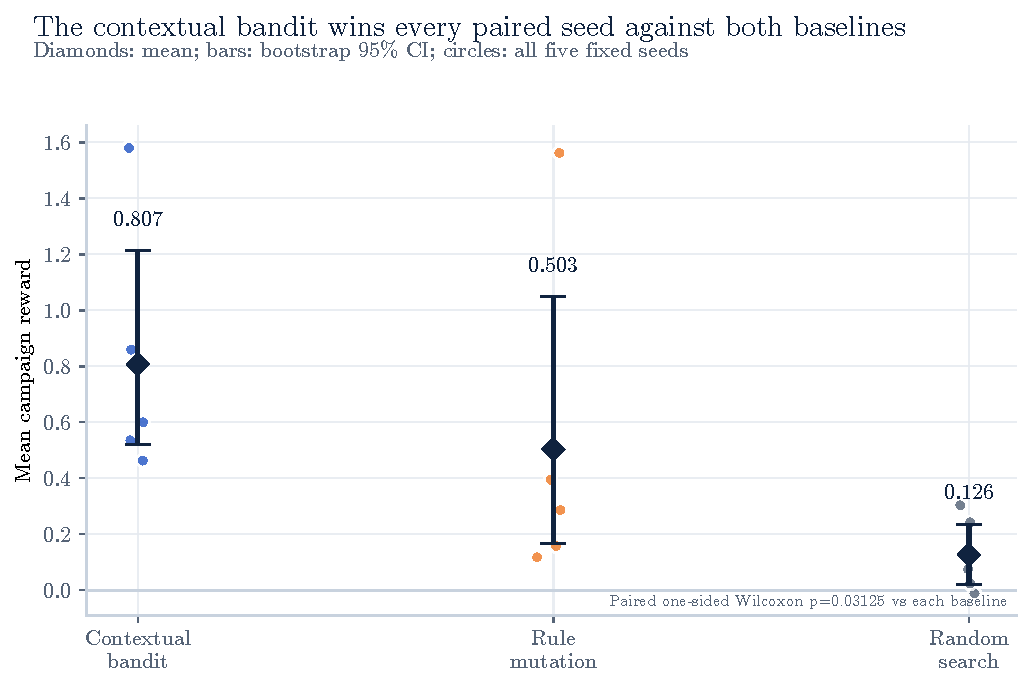
\includegraphics[width=0.92\linewidth]{fig03_reward_comparison.pdf}
  \caption[Equal-budget reward comparison]{Equal-budget reward comparison. All five fixed seeds are shown as individual points; bars are five-seed means and error bars are bootstrap 95\% CIs. No single seed is promoted as the result.\evidence{E1,E2}}
  \label{fig:reward}
\end{figure}

\Cref{fig:reward} shows that the bandit mean exceeds both baselines, while the individual points show the dispersion hidden by the mean. H1 is supported: all five paired seeds favor LinUCB over random and rule mutation, with one-sided paired Wilcoxon $p=0.03125$ for each comparison. This result supports adaptive search under the fixed budget; it does not imply an order-of-magnitude universal advantage.

\subsection{H2: held-out efficacy improves through V2}
\begin{figure}[H]
  \centering
  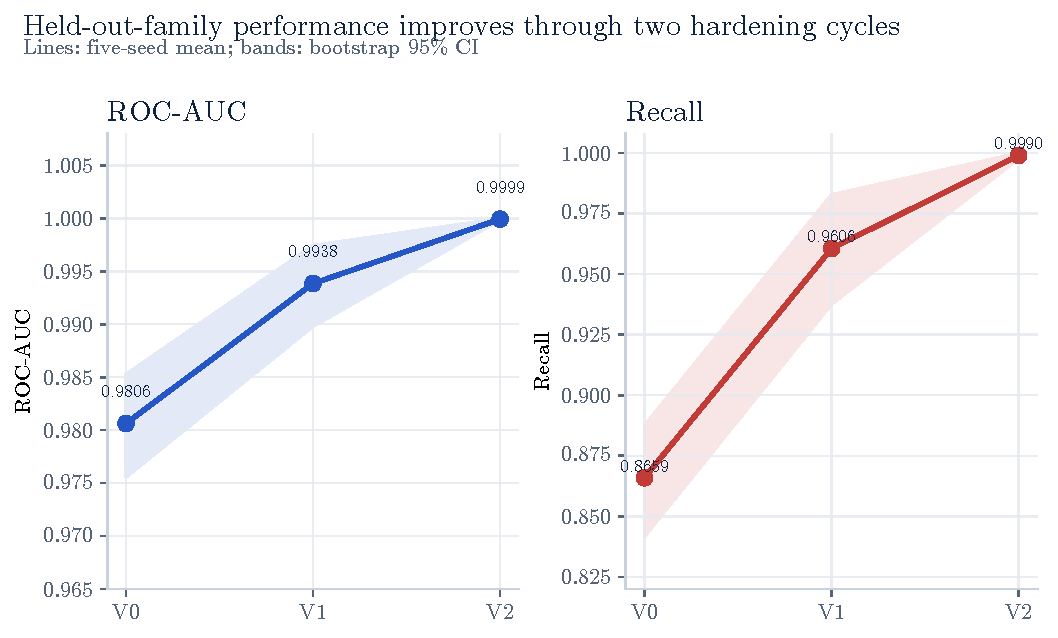
\includegraphics[width=0.94\linewidth]{fig04_defender_progression.pdf}
  \caption[Held-out efficacy progression]{Held-out ROC-AUC and recall progression. Lines are five-seed means and shaded bands are bootstrap 95\% CIs. Each generation is calibrated independently on validation data; test FPRs are observed, not forced to match.\evidence{E1,E3}}
  \label{fig:defender}
\end{figure}

\begin{table}[H]
\centering\small
\begin{tabular}{lccc}
\toprule
\textbf{Metric} & \textbf{V0 mean $\pm$ SD} & \textbf{V1 mean $\pm$ SD} & \textbf{V2 mean $\pm$ SD} \\
\midrule
ROC-AUC & $0.9806\pm0.0062$ & $0.9938\pm0.0049$ & $0.99993\pm0.00010$ \\
Recall & $86.59\%\pm2.91\%$ & $96.06\%\pm2.92\%$ & $99.90\%\pm0.15\%$ \\
Precision at experiment prevalence & $90.68\%\pm1.92\%$ & $90.73\%\pm1.06\%$ & $91.28\%\pm1.72\%$ \\
Legitimate test FPR & $0.911\%\pm0.163\%$ & $1.007\%\pm0.111\%$ & $0.982\%\pm0.200\%$ \\
\bottomrule
\end{tabular}
\fixedtablecaption{tab:efficacy}{7}{Held-out-family results. Each threshold is calibrated independently on validation at a 1\% target FPR; test FPRs are natural realizations.\evidence{E1,E3}}
\end{table}

The rising AUC and recall in \cref{fig:defender} support H2 within this synthetic protocol. The legitimate test FPRs differ by generation even though validation calibration targets 1\%; this is expected sampling variation and demonstrates that the test set was not used to force a common operating point.

\subsection{H3: later-generation stability is directional, not conclusive}
\begin{figure}[H]
  \centering
  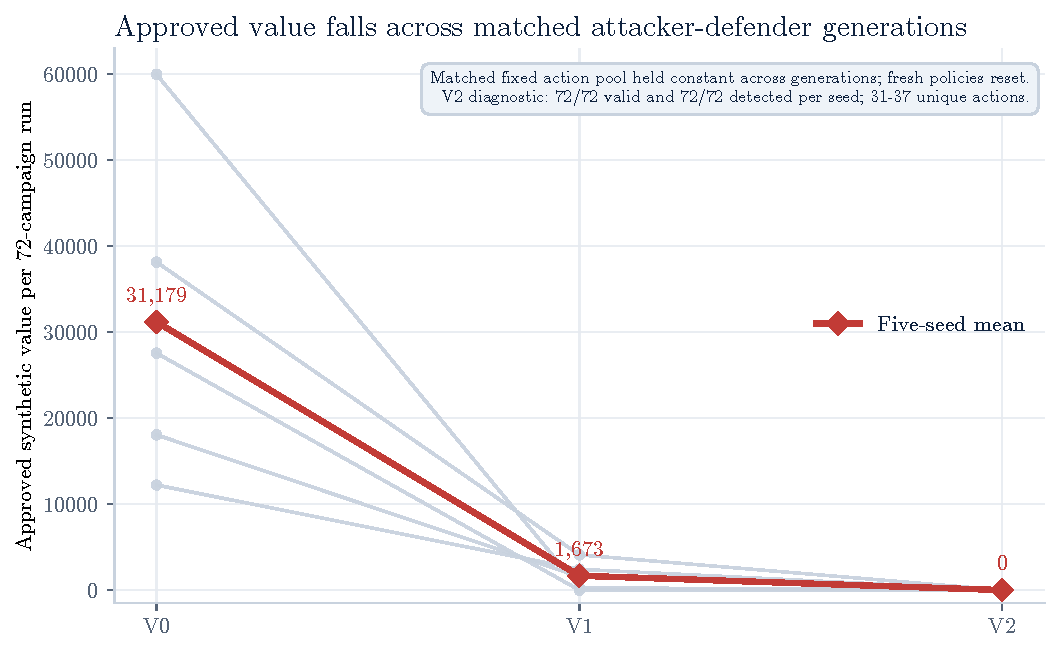
\includegraphics[width=0.92\linewidth]{fig05_fresh_approved_value.pdf}
  \caption[Fresh-attacker approved value]{Fresh-attacker approved synthetic value across defender generations. The chart annotates the matched-pool boundary directly: actions and random streams are held constant across V0, V1 and V2.\evidence{E1,E2,E5}}
  \label{fig:value}
\end{figure}

\begin{evidencebox}
Against a matched, fixed action pool held constant across generations, the hardened defender (V2) detected every campaign across five seeds.
\end{evidencebox}

The underlying artifact contains 360/360 valid campaigns, 360/360 fully detected campaigns and zero approved value; each seed selects 31--37 unique actions. This is not evidence about an independently resampled V2 action space, unbounded adversaries or live traffic.\evidence{E5}

The V1--V2 reward comparison is lower on four seeds and tied on one, with one-sided paired Wilcoxon $p=0.0625$. H3 is directionally supported but not confirmed. The evidence shows no observed oscillation through one additional generation pair; it does not eliminate the instability risk identified in the Adyen study.\evidence{E1,E2}\cite{vangara2024contextual}

\subsection{H4: novelty contribution is rejected}
Novelty-on minus novelty-off reward is -0.017 (95\% CI -0.137 to 0.121; two-sided paired Wilcoxon $p=0.625$). H4 is rejected: the novelty term is not a demonstrated driver of attacker quality. The complete numerical ablation is reported once in \tableref{tab:ablation}{2}; the interpretation is intentionally shown beside the positive efficacy results.\evidence{E1,E2}

\subsection{Prevalence is the operational boundary}
\begin{figure}[H]
  \centering
  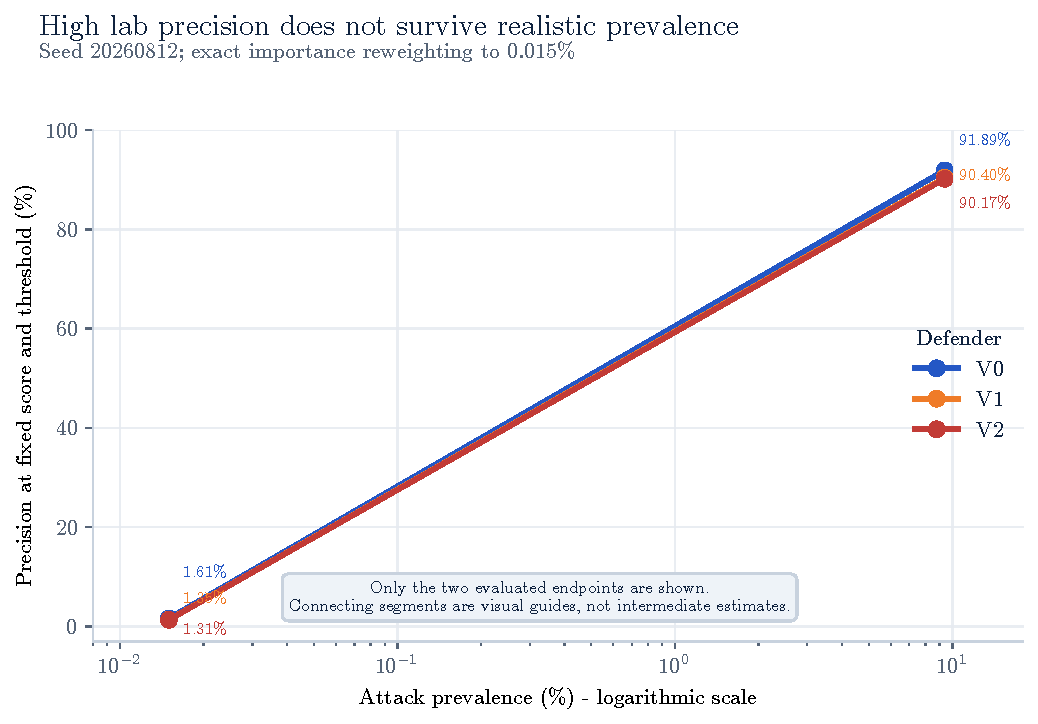
\includegraphics[width=0.94\linewidth]{fig06_precision_prevalence.pdf}
  \caption[Precision versus prevalence]{Precision versus prevalence. Only the two artifact-backed endpoints are measured; connecting segments are labeled as visual interpolation only. Results are seed-20260812-specific; the full range appears in Appendix Table A3.\evidence{E4}}
  \label{fig:prevalence}
\end{figure}

\begin{boundarybox}
For V2, precision falls from 90.17\% at 9.39\% experimental prevalence to 1.31\% at exactly reweighted 0.015\% prevalence (seed 20260812; full range in Appendix Table A3). AUC and FPR remain fixed for the same scores and threshold; precision changes because false positives vastly outnumber true positives when fraud is rare. The lab precision must not be presented as a production estimate.\evidence{E4}
\end{boundarybox}

\section{Real-World Feasibility and Business Impact}
\sectionlead{The feasible product is an offline adversarial assurance layer that feeds governed challenger development - not an autonomous attacker and not a replacement for network decisioning.}

\begin{table}[H]
\centering\small
\begin{tabularx}{\linewidth}{L{25mm}YY}
\toprule
\textbf{Stage} & \textbf{Production interface} & \textbf{Control or evidence} \\
\midrule
1. Observe & Approved outcome labels, feature contracts and drift summaries & No raw cardholder data enters the synthetic lab by default \\
2. Model & Parameterize the digital twin from authorized aggregates & Versioned scenarios, lineage and fidelity tests \\
3. Challenge & Attack frozen champion or challenger snapshots offline & Equal budgets, validity firewall and reproducible seeds \\
4. Harden & Export valid evasions and feature-gap findings & Human approval, validation recalibration and model-risk review \\
5. Release & Shadow or champion-challenger deployment & Kill switch, drift and false-positive monitoring \\
\bottomrule
\end{tabularx}
\fixedtablecaption{tab:deployment}{8}{Directional deployment path. This is an architectural proposal, not measured implementation performance.\evidence{E7}}
\end{table}

\subsection{Integration path}
AegisLoop can sit upstream of an issuer's model-development environment. It consumes governed schemas, calibrated aggregate constraints and frozen model APIs; it returns scenario DSL versions, campaign diagnostics, evasive examples and proposed feature gaps. The online score remains owned by existing authorization infrastructure.\evidence{E7}

\subsection{Scalability}
Campaign evaluation is embarrassingly parallel across action candidates and seeds, while policy updates are lightweight linear algebra. The scenario DSL isolates research expansion from detector code. A credible scale-up plan is therefore to distribute simulator rollouts, retain deterministic seeds and promote only versioned aggregates across governance boundaries. No latency or throughput number is claimed because this prototype has not been benchmarked as production infrastructure.

\subsection{Commercial value levers}
The business case has four measurable levers: fraud loss avoided through earlier discovery, false-decline cost avoided through better calibrated controls, analyst effort reduced through prioritized evasions, and model-release risk reduced through repeatable adversarial tests. The evidence supports the mechanism, not an ROI estimate; portfolio loss rates, review costs and authorization economics must be supplied by the deployment partner before monetization is quantified.

\subsection{Alignment with Mastercard's public direction}
Decision Intelligence Pro publicly emphasizes relationship-aware, contextual and real-time risk assessment. AegisLoop is complementary: it creates governed synthetic pressure tests for the entity and intent signals that a decision engine may consume. This is a directional comparison only; no equivalence to Mastercard's technology or published performance is asserted.\cite{mastercard2024dipro}

\section{Limitations and Responsible Use}
\sectionlead{AegisLoop has earned a strong laboratory result, not a production performance claim; the remaining gaps are explicit enough to form the next validation agenda.}

\begin{description}[leftmargin=0pt,labelindent=0pt,style=nextline,font=\bfseries]
  \item[Synthetic-only evidence.] The simulator has no authorized real reference corpus, so structural validity cannot establish statistical or behavioral equivalence to a live portfolio. External validation must compare entity-level temporal and graph signatures.\evidence{E7}\cite{sajja2026synthetic}
  \item[Matched-pool V2 scope.] The V2 claim holds against a matched, fixed action pool shared across generations. It does not establish resistance to an independently resampled, larger or open-ended attack space.\evidence{E5}
  \item[Small seed count.] Five paired seeds allow an exact one-sided $p=0.03125$ only when every difference has the expected sign. Confidence intervals remain wide for attacker reward.\evidence{E1,E2,E8}
  \item[Limited stability horizon.] Only V0--V1--V2 is observed. The V1--V2 reward result is directional at $p=0.0625$; additional generations are required to test oscillation.\evidence{E1}\cite{vangara2024contextual}
  \item[Prevalence transfer.] Experiment prevalence is 9.39\% in the seed-20260812 held-out slice. Exact reweighting shows precision near 1.3\%--1.6\% at 0.015\%, so production thresholds and review capacity require portfolio calibration.\evidence{E4}
  \item[No live-operational proof.] The prototype has no live endpoints, no measured production latency, no model-risk approval and no measured ROI. Deployment claims are architectural and qualitative.\evidence{E7}
\end{description}

\subsection{Responsible-use controls}
\begin{itemize}
  \item Keep the red-team policy inside a synthetic, access-controlled environment with no live payment-rail connector.
  \item Use only synthetic, anonymized or explicitly authorized inputs consistent with the competition rules.\competition
  \item Require human approval before an evasion enters training or a challenger model reaches shadow deployment.
  \item Publish negative results and provenance beside performance summaries so presentation cannot outrun evidence.
\end{itemize}

\section{Conclusion}
\sectionlead{AegisLoop's defensible novelty is a campaign-level extension of single-transaction RL fraud-evasion attacks that closes the loop into adversarial defender hardening.}

The solution converts the challenge's Identify-Generate-Defend brief into one governed feedback system. Eight equal-priority archetypes define the search space; a stateful entity-linked simulator generates campaigns; a contextual bandit finds blind spots more effectively than equal-budget random and rule baselines; and a leakage-controlled ensemble improves across two hardening cycles.\competition\evidence{E1--E8}

The evidence is strongest where it is most bounded. The five-seed bandit advantage is paired and statistically positive. Held-out AUC and recall improve through V2. The V2 matched-pool diagnostic is non-trivial because every campaign is valid and action use remains diverse. At the same time, the novelty bonus does not help, later-generation stability is not conclusive, and realistic prevalence collapses precision. Those are not presentation defects; they are the difference between an innovation demo and an auditable model-development instrument.\evidence{E1--E5}

\begin{evidencebox}
The next decision is therefore concrete: validate the digital twin against authorized aggregate behavioral signatures, expand the independently sampled action space and generation horizon, then evaluate the resulting challenger in shadow mode with portfolio-specific calibration. Until that evidence exists, AegisLoop should be positioned exactly as built - an offline adaptive fraud-defense laboratory.
\end{evidencebox}

\clearpage
\printbibliography[title={References}]

\appendix
\section{Full Statistical Tables}

\subsection{Raw seed-level outcomes}
\begin{landscape}
\begin{table}[p]
\centering\scriptsize
\resizebox{0.95\linewidth}{!}{\begin{tabular}{lrrrrrrrrr}
\toprule
\textbf{Seed} & \textbf{Bandit} & \textbf{Rule} & \textbf{Random} & \textbf{V0 AUC} & \textbf{V1 AUC} & \textbf{V2 AUC} & \textbf{V0 value} & \textbf{V1 value} & \textbf{V2 value} \\
\midrule
20260812 & 1.579 & 1.562 & 0.303 & 0.9886 & 0.9961 & 0.99979 & 59,952 & 267 & 0 \\
20260813 & 0.859 & 0.286 & 0.242 & 0.9724 & 0.9867 & 1.00000 & 38,133 & 4,100 & 0 \\
20260814 & 0.463 & 0.157 & -0.011 & 0.9772 & 0.9928 & 0.99984 & 27,549 & 0 & 0 \\
20260815 & 0.535 & 0.394 & 0.074 & 0.9815 & 1.0000 & 1.00000 & 12,214 & 2,417 & 0 \\
20260816 & 0.599 & 0.117 & 0.024 & 0.9834 & 0.9936 & 1.00000 & 18,048 & 1,579 & 0 \\
\bottomrule
\end{tabular}}
\caption*{Table A1. Raw seed-level primary outcomes. Source: \texttt{seed\_results.csv}. ``Value'' is fresh-attacker approved synthetic value.\evidence{E2}}
\end{table}
\end{landscape}

\subsection{Calibration audit}
\begin{table}[H]
\centering\small
\resizebox{0.98\linewidth}{!}{\begin{tabular}{lrrrrr}
\toprule
\textbf{Defender} & \textbf{Source split} & \textbf{Rows} & \textbf{Target FPR} & \textbf{Validation FPR} & \textbf{Threshold} \\
\midrule
V0 & legitimate validation 60--80\% & 5,600 & 1.00\% & 1.00\% & 0.138344 \\
V1 & legitimate validation 60--80\% & 5,600 & 1.00\% & 1.00\% & 0.136563 \\
V2 & legitimate validation 60--80\% & 5,600 & 1.00\% & 1.00\% & 0.138693 \\
\bottomrule
\end{tabular}}
\caption*{Table A2. Calibration audit. Validation-test event-ID overlap is zero and test rows used for threshold selection is false.\evidence{E3}}
\end{table}

\subsection{Seed-20260812 prevalence metrics}
\begin{landscape}
\begin{table}[p]
\centering\scriptsize
\resizebox{0.95\linewidth}{!}{\begin{tabular}{llrrrrrrr}
\toprule
\textbf{Defender} & \textbf{Scenario} & \textbf{Prevalence} & \textbf{Fraud rows} & \textbf{Repeats} & \textbf{ROC-AUC} & \textbf{Precision} & \textbf{Recall} & \textbf{FPR} \\
\midrule
V0 & Experiment & 9.3851\% & 580 & 1 & 0.9886 & 91.89\% & 89.83\% & 0.821\% \\
V0 & Literal downsample & 0.0179\% & 1 & 400 & 0.9843 & 1.91\% & 89.75\% & 0.821\% \\
V0 & Exact reweight & 0.0150\% & 580 & 1 & 0.9886 & 1.61\% & 89.83\% & 0.821\% \\
V1 & Experiment & 9.3851\% & 580 & 1 & 0.9961 & 90.40\% & 97.41\% & 1.071\% \\
V1 & Literal downsample & 0.0179\% & 1 & 400 & 0.9931 & 1.59\% & 97.25\% & 1.071\% \\
V1 & Exact reweight & 0.0150\% & 580 & 1 & 0.9961 & 1.35\% & 97.41\% & 1.071\% \\
V2 & Experiment & 9.3851\% & 580 & 1 & 0.9998 & 90.17\% & 99.66\% & 1.125\% \\
V2 & Literal downsample & 0.0179\% & 1 & 400 & 0.9997 & 1.55\% & 99.50\% & 1.125\% \\
V2 & Exact reweight & 0.0150\% & 580 & 1 & 0.9998 & 1.31\% & 99.66\% & 1.125\% \\
\bottomrule
\end{tabular}}
\caption*{Table A3. Seed-20260812 prevalence metrics. Exact-reweight rows support the standalone claims. Literal downsampling uses one fraud row per repeat and is a high-variance sensitivity check.\evidence{E4}}
\end{table}
\end{landscape}

\subsection{V2 campaign diagnostics by seed}
\begin{table}[H]
\centering\scriptsize
\begin{tabular}{lrrrrrrrrr}
\toprule
\textbf{Seed} & \textbf{Campaigns} & \textbf{Valid} & \textbf{Detected} & \textbf{Events} & \textbf{Value} & \textbf{Mean $F$} & \textbf{Min $F$} & \textbf{Actions} & \textbf{Families} \\
\midrule
20260812 & 72 & 72 & 72 & 864 & 0.0 & 0.9266 & 0.8369 & 33 & 6 \\
20260813 & 72 & 72 & 72 & 864 & 0.0 & 0.9178 & 0.8376 & 32 & 6 \\
20260814 & 72 & 72 & 72 & 864 & 0.0 & 0.9193 & 0.8238 & 37 & 6 \\
20260815 & 72 & 72 & 72 & 864 & 0.0 & 0.9269 & 0.8371 & 31 & 6 \\
20260816 & 72 & 72 & 72 & 864 & 0.0 & 0.9244 & 0.8307 & 37 & 6 \\
\bottomrule
\end{tabular}
\caption*{Table A4. V2 campaign diagnostics by seed. Source: \texttt{v2\_campaign\_diagnostics.csv}, artifact version 1.0.\evidence{E5}}
\end{table}

\section{Reproducibility and Evidence Ledger}
\subsection{Reproduce the evidence}
\begin{lstlisting}[style=aegiscode]
.venv\Scripts\python -m pytest
.venv\Scripts\python -m ruff check src experiments tests app.py scripts
.venv\Scripts\python experiments\run_multiseed.py --seeds 20260812,20260813,20260814,20260815,20260816
.venv\Scripts\python scripts\make_figures.py --print-pdf --output-dir deliverables/latex/paper/figures
\end{lstlisting}
The full multi-seed command writes \texttt{seed\_results.csv}, \texttt{aggregate.json} and the versioned V2 diagnostic. The figure script reads approved artifacts and emits vector PDFs plus a hash-and-value manifest. This LaTeX paper includes those vector outputs; no result is copied from an earlier withdrawn headline.\evidence{E1--E5,E8}

\begin{evidencebox}
\textbf{Repository:} \url{https://github.com/Hermes-25/AegisLoop}\\
\textbf{Working prototype:} \url{https://aegisloop-mcic-2026.vercel.app}\\
\textbf{Public paper:} \url{https://aegisloop-mcic-2026.vercel.app/AegisLoop_Solution_Walkthrough.pdf}
\end{evidencebox}

\subsection{Approved evidence ledger}
\small
\begin{tabularx}{\linewidth}{L{10mm}L{62mm}Y}
\toprule
\textbf{ID} & \textbf{Path} & \textbf{What it supports} \\
\midrule
E1 & \path{artifacts/full_multiseed/aggregate.json} & Five-seed means, SDs, CIs and significance tests \\
E2 & \path{artifacts/full_multiseed/seed_results.csv} & Raw per-seed outcomes \\
E3 & \path{artifacts/precomputed/calibration_audit.json} & Temporal split, threshold source and leakage audit \\
E4 & \path{artifacts/precomputed/prevalence_metrics.csv} & Seed-20260812 prevalence scenarios and metrics \\
E5 & \path{artifacts/precomputed/v2_campaign_diagnostics.csv} & V2 validity, detection, fidelity, reward decomposition and action diversity \\
E6 & \path{artifacts/precomputed/attack_atlas.json} & Eight archetypes, 32 variants and scenario metadata \\
E7 & \path{docs/ARCHITECTURE.md} & System, simulator, reward and deployment architecture \\
E8 & \path{docs/BENCHMARKS.md} & Protocol contract, statistics and full-versus-quick distinction \\
E9 & \path{RESULTS.md} & Phase 1 verified narrative and result tables \\
E10 & \path{PHASE1_CHANGELOG.md} & Finding-to-remediation changelog \\
\bottomrule
\end{tabularx}
\normalsize

\subsection{Evidence-tag convention}
Literature citations are managed by \texttt{biblatex} and appear as ordinary numeric references. Superscript tags E1--E10 refer only to versioned project evidence in the ledger above; C1 refers to the private competition rules copied into \texttt{Comp\_Rules\_Overview.txt}. This separation prevents internal evidence identifiers from colliding with scholarly citations.

\end{document}
